\documentclass[a4paper]{article}

%%% usepackage %%%
\usepackage{color}
\usepackage{ulem}
\usepackage{amsmath}
\usepackage{amssymb}
\usepackage{xfrac}
\usepackage{import}
\usepackage{listings}
\usepackage{hyperref}
\usepackage{float}
\usepackage[inner=2cm, outer=2cm, top=2cm, bottom=2cm]{geometry}
\usepackage{xepersian}
\settextfont{Dubai}
\fontsize{40}{18}\selectfont
\usepackage{eso-pic}% http://ctan.org/pkg/eso-pic
\usepackage{lipsum}% http://ctan.org/pkg/lipsum

%%% define color %%%
\definecolor{codegreen}{rgb}{0,0.6,0}
\definecolor{codegray}{rgb}{0.5,0.5,0.5}
\definecolor{codepurple}{rgb}{0.58,0,0.82}
\definecolor{backcolour}{rgb}{0.95,0.95,0.92}

\definecolor{dkgreen}{rgb}{0,0.6,0}
\definecolor{gray}{rgb}{0.5,0.5,0.5}
\definecolor{mauve}{rgb}{0.58,0,0.82}

\def\ojoin{\setbox0=\hbox{$\bowtie$}%
  \rule[-.02ex]{.25em}{.4pt}\llap{\rule[\ht0]{.25em}{.4pt}}}
\def\leftouterjoin{\mathbin{\ojoin\mkern-5.8mu\bowtie}}
\def\rightouterjoin{\mathbin{\bowtie\mkern-5.8mu\ojoin}}
\def\fullouterjoin{\mathbin{\ojoin\mkern-5.8mu\bowtie\mkern-5.8mu\ojoin}}

\lstset{frame=tb,
  language=SQL,
  aboveskip=3mm,
  belowskip=3mm,
  showstringspaces=false,
  columns=flexible,
  basicstyle={\small\ttfamily},
  numbers=none,
  numberstyle=\tiny\color{gray},
  keywordstyle=\color{blue},
  commentstyle=\color{dkgreen},
  stringstyle=\color{mauve},
  breaklines=true,
  breakatwhitespace=true,
  tabsize=3
}


%%% newcommand %%%
\newcommand{\nn}{\textcolor{red}{\textbf{NOT NULL}}}
\newcommand{\emailone}{\texttt{abbas.yazdanmehr1@gmail.com}}
\newcommand{\fulltitle}[2]{\title{#1 \\ #2}}
\newcommand{\myinf}{
	\author{\noindent
عباس یزدان مهر
\\
99243077\\
 مهندسی کامپیوتر, دانشگاه شهید بهشتی
\\
\emailone
	}
}
\newcommand{\goodby}{\begin{center}{\huge
پایان
}\end{center}}



\begin{document}

\fulltitle{
پایگاه داده
}{
تمرین چهارم
}

\myinf

\maketitle

\newpage


\myinf
\section{}
\subsection*{الف}

\begin{latin}
  \begin{table}[H]
    \begin{small}
      \begin{center}
        \begin{tabular}[c]{|l|l|}
          \hline
          Entity Set & Primary Key \\
          \hline
          \hline
          author(name, address, URL) & name \\
          \hline
          book(ISBN, title, year, price) & ISBN \\
          \hline
          publisher(name, address, phone, URL) & name \\
          \hline
          customer(email, name, address, phone) & email \\
          \hline
          warehouse(code) & code \\
          \hline
          shopping\_basket(basket\_id) & Basket\_id (not explicit)\\
          \hline
        \end{tabular}
      \end{center}
    \end{small}
  \end{table}
  
\end{latin}

\subsection*{ب}
چون فیلم هم می تواند قابل دانلود باشد و هم میتواند بصورت دیسکی
باشد باید از overlapping generalization استفاده کنیم. 

\begin{figure} [H]
  \begin{small}
    \begin{center}
      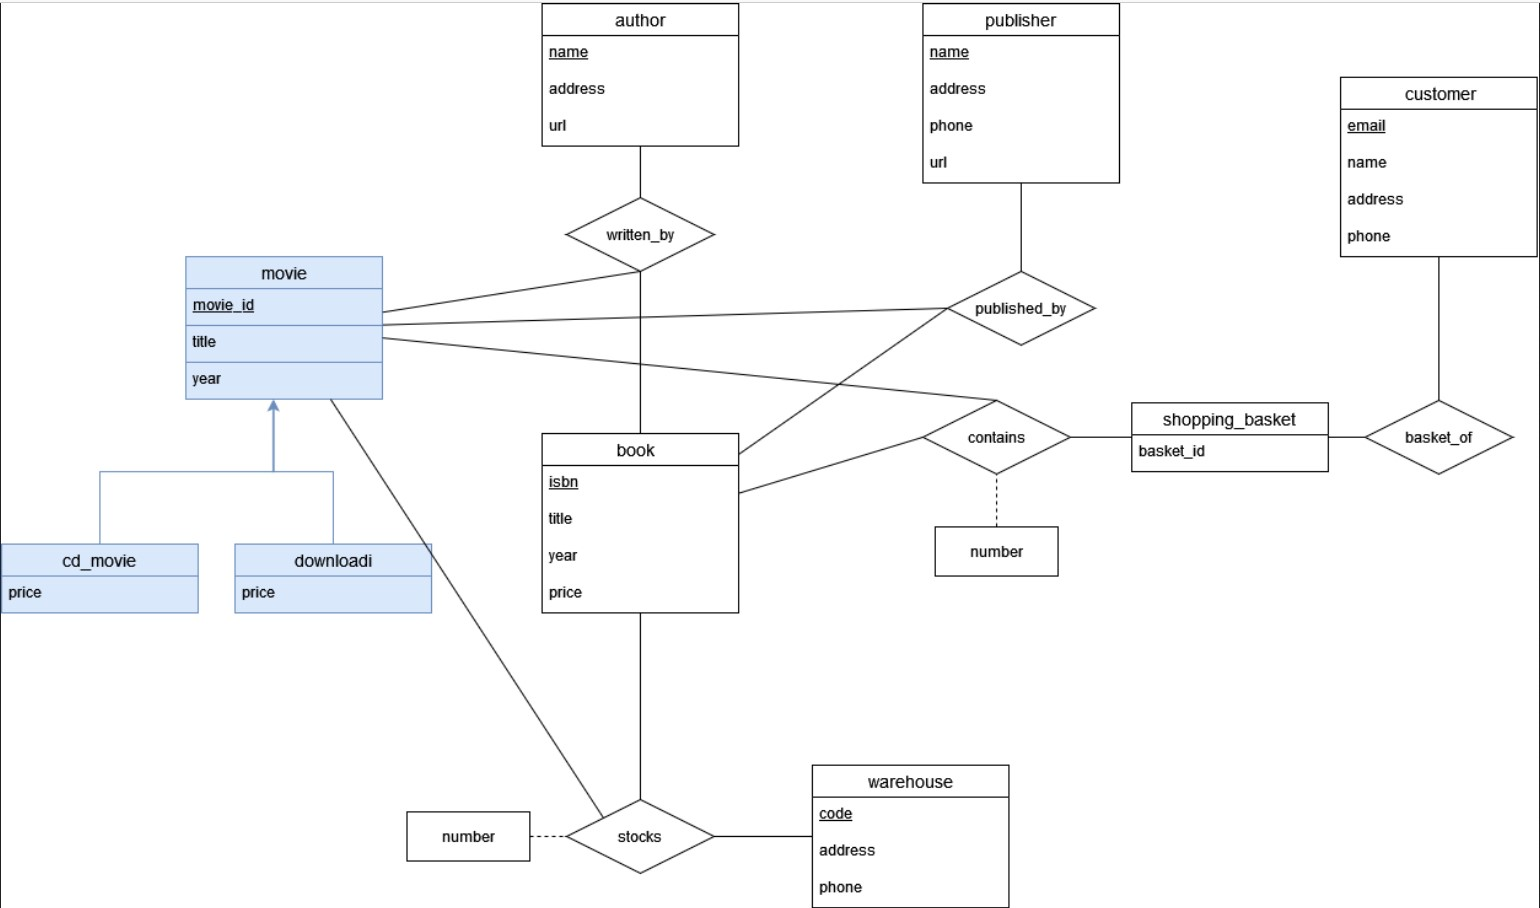
\includegraphics[width=0.95\textwidth]{figures/1.jpg}
    \end{center}
  \end{small}
\end{figure}

\subsection*{نکته}
در شکل movie و book باهم در یک رابطه شرکت نمی کند و فقط یکی شرکت می کند.

\newpage
\myinf
\subsection*{ج}
\begin{figure} [H]
  \begin{small}
    \begin{center}
      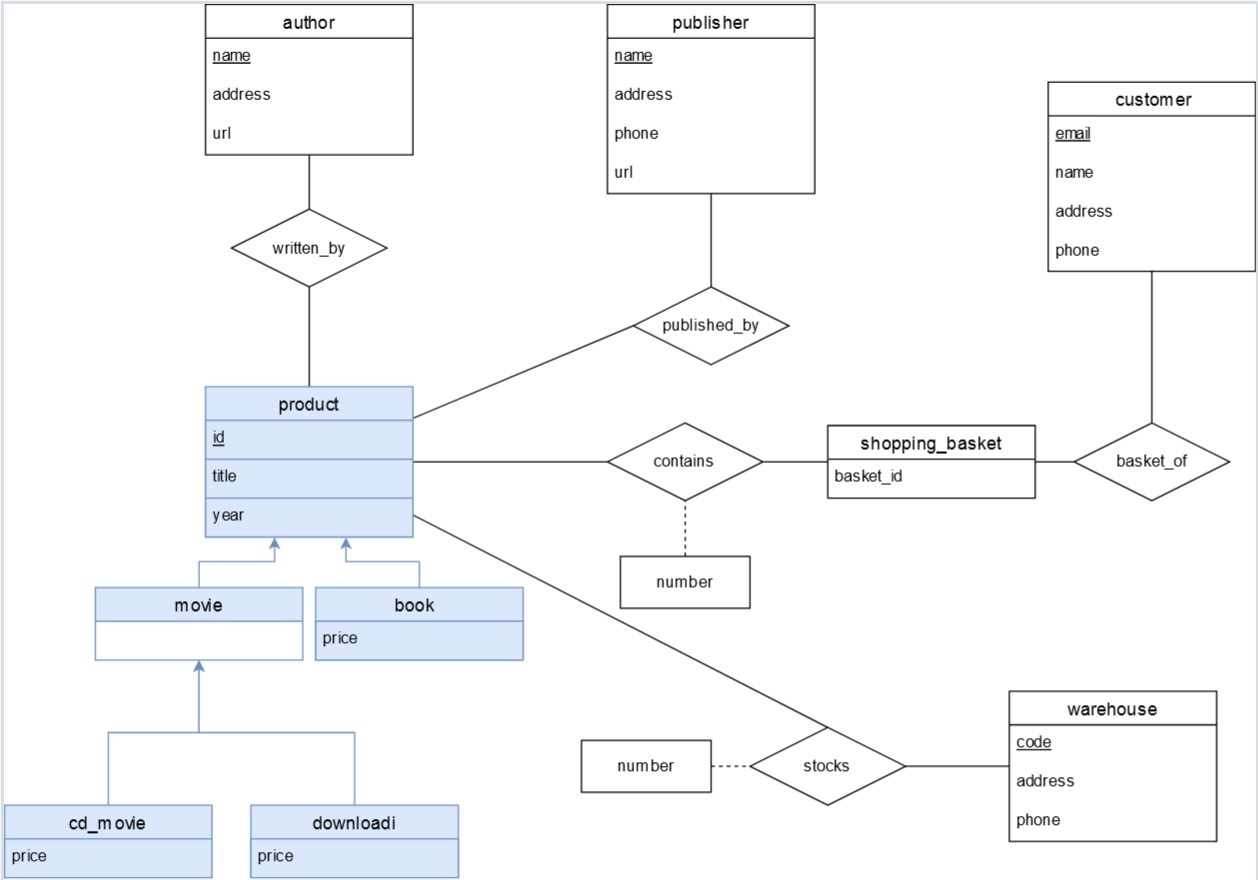
\includegraphics[width=0.95\textwidth]{figures/1-j.jpg}
    \end{center}
  \end{small}
\end{figure}

\newpage
\myinf
\section{}
\begin{figure}[H]
  \begin{small}
    \begin{center}
      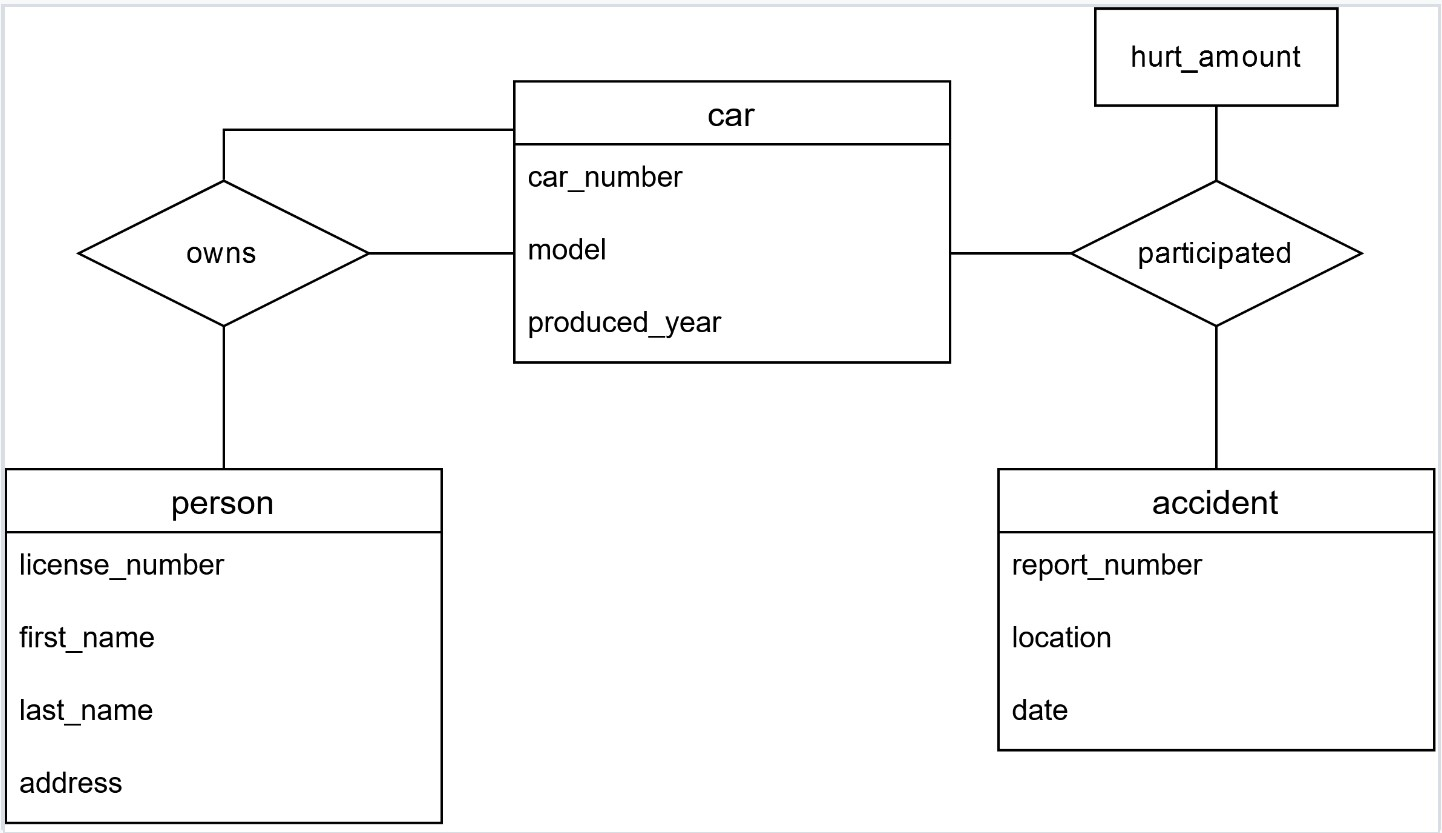
\includegraphics[width=0.95\textwidth]{figures/2.jpg}
    \end{center}
  \end{small}
\end{figure}

\newpage
\myinf
\section{}
موجودیت strong  خودش حتما کلید اصلی دارد،
و به دیگر موجودیت ها وابسته نیست و با یک مستطیل
نمایش داده می شود،
ولی موجودیت weak کلیدش را از موجودیت های قوی میگیرد که به آنها discriminator می گویند، و به آنها
وابسته است 
و با یک مستطیل دوخطی نمایش داده میشود.

\section{}
\begin{enumerate}
  \item
   در پایگاه داده بهتر است هر موجودیت ویژگی های خاص
خود را داشته باشد،
در صورتی که فقط از strong استفاده کنیم، 
باید ویژگی های مربوط به موجودیت هایی که به آن وابسته ایم
را هم در موجودیت وابسته بیاوریم که باعث میشود
اطلاعات تکراری داشته باشیم.

  \item
استفاده از موجودیت ضعیف باعث میشود که یک موجودیت به
چند موجودیت وابسته شود و این باعث می شود
که سرعت عملیات ها بیشتر باشد و در ضمن 
محدودیت هایی ایجاد می کند که باعث می شود از خطاها جلوگیری
شود.
\end{enumerate}

\section{}
شماتیک جداول:
\begin{latin}
  \noindent
  {\Large convention: }\textit{table\_name}(\emph{\textbf{primary\_key}}, \dashuline{\textbf{foreign\_key}}(references), simple\_attribute,) \\[1cm]
  \noindent
  \textit{employee\_name}(\emph{\textbf{name\_id}}, fname, minit, lname) \\
  \textit{employee}(\emph{\textbf{ssn}}, \dashuline{\textbf{name\_id}}, sex, address, salary, bdate, \\
  \dashuline{\textbf{department.name \nn, department.number \nn}}, \\
  \dashuline{\textbf{supervisor\_ssn}}(employee.ssn), \dashuline{\textbf{supervisee\_ssn}}(employee.ssn)) \\
  \textit{project}(\emph{\textbf{name, number}}, location, \dashuline{\textbf{department.name, department.number}}) \\
  \textit{department}(\emph{\textbf{name, number}}, number\_of\_employee) \\
  \textit{dependent}(\emph{\dashuline{\textbf{employee.name\_id \nn}}}, sex, birth\_date, relationship) \\
  \textit{manages}(\emph{\dashuline{\textbf{ssn, department.name \nn, department.number \nn}}}, start\_date) \\
  \textit{works\_on}(\emph{\dashuline{\textbf{ssn \nn, project.name \nn, project.number \nn}}}, hours) \\  
  \textit{department\_locations}(\emph{\dashuline{\textbf{department.name, department.number}}, \textbf{location}})

\end{latin}

\newpage
\myinf
\section{}
همه ی این موارد مربوط به قسمت ارتباط بین سطح بالا و سطح پایین در specialization 
است.
\\
همه ی  این موارد جزء موارد محدود سازی ER هستند.
\\
 در صورتی که specialization به صورت disjoint باشد
 یک موجودیت تنها می تواند به یک موجودیت که در سطح
 پایین تری  قرار دارد رابطه داشته باشد که یعنی هر
 کلاس پدر تنها می تواند به یک زیرکلاس یا کلاس فرزند
 مرتبط باشد و نه هر
 دو. مثلا یک موجودیت پدر با نام ماشین یا میتواند
  مرتبط با موجودیت ماشین سنگین باشد یا موجودیت ماشین سبک
  و نه هردو.
\\
در صورتی که specialization به صورت overlapping باشد
برعکس disjoint است به این صورت که هر موجودیت
میتواند به یک یا چند موجودیت که زیرکلاس آن هستند
مرتبط شوند. مثلا یک موجودیت با نام شخص هم میتواند
به موجودیت کارمند مرتبط شود و هم به موجودیت دانشجو.
\\

\subsubsection*{مقایسه}
در disjoint هر موجودیت سطح بالا فقط به یک موجودیت
سطح پایین مرتبط می شود ولی در overlapping تعداد ارتباط
با زیرکلاس ها محدودیتی ندارد.
\\ \\
در یک specialization total یک موجودیت سطح بالاتر حتما باید به یک موجودیت سطح پایین تر مرتبط باشد.
\\
در یک specialization partial یک موجودیت سطح بالا حتما نبای د به یک موجودیت سطح پایین تر مرتبط باشد 
باشد بلکه میتواند ارتباطی نداشته باشد. 

\subsubsection*{مقایسه}
پس specialization total حتما هر موجودیت سطح بالاتر 
به یک موجودیت پایین تر مرتبط است اما در partial لزومی ندارد.

\newpage
\myinf
\section{}

\begin{figure}[H]
  \begin{small}
    \begin{center}
      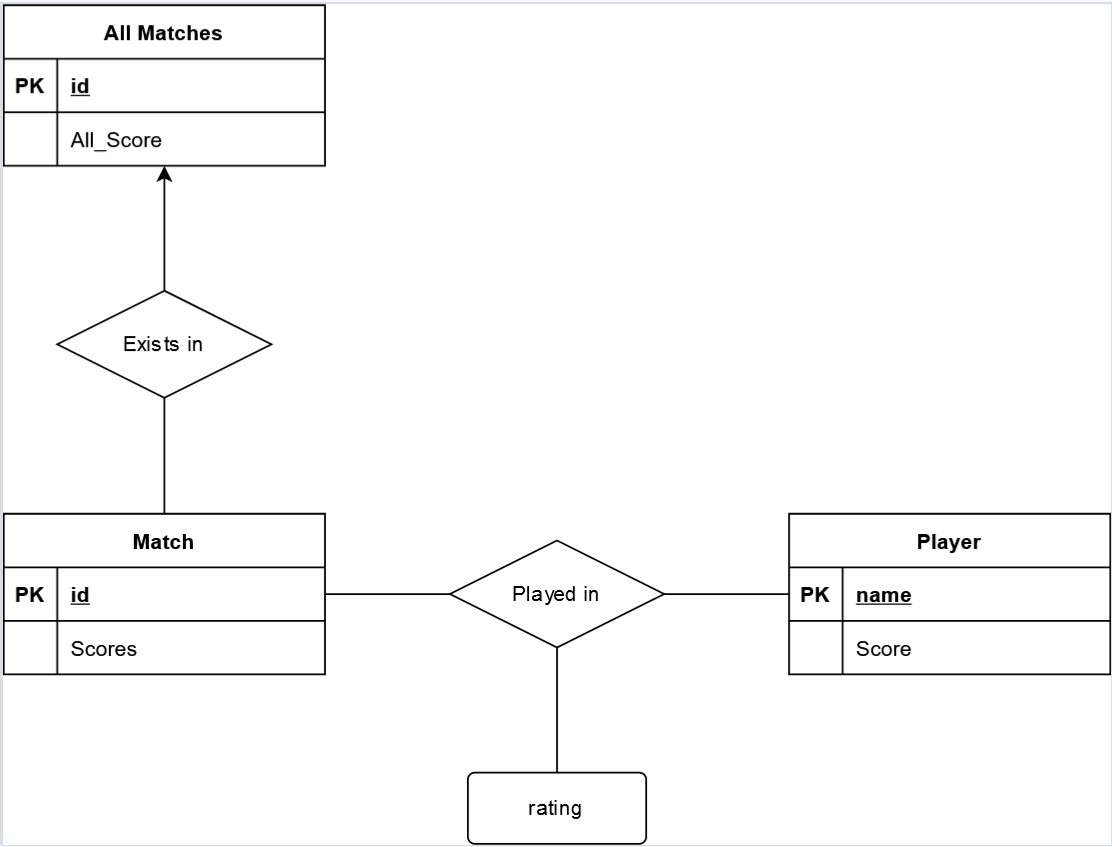
\includegraphics[width=0.95\textwidth]{figures/7.jpg}
    \end{center}
  \end{small}
\end{figure}

\section{}

شماتیک جداول:
\begin{latin}
  \noindent
  {\Large convention: }\textit{table\_name}(\emph{\textbf{primary\_key}}, \dashuline{\textbf{foreign\_key}}(references), simple\_attribute,) \\[1cm]
  \noindent
  \textit{student}(\emph{\textbf{student\_id}}, student\_name, dob, age, door\_number, street, city, state, pin) \\
  \textit{course}(\emph{\textbf{course\_id}}, course\_name) \\
  \textit{subjects}(\emph{\textbf{subject\_id}}, subject\_name, \dashuline{\textbf{lecturer\_id}}, \dashuline{\textbf{course\_id}}) \\
  \textit{lecturer}(\emph{\textbf{lecturer\_id}}, lecturer\_name, \dashuline{\textbf{course\_id}}, \dashuline{\textbf{student\_id}}) \\
  \textit{attends}(\emph{\textbf{\dashuline{student\_id}, \dashuline{course\_id}}}) \\
  \textit{takes}(\emph{\textbf{\dashuline{lecturer\_id}, \dashuline{course\_id}}}) \\
  \textit{hobby}(\emph{\textbf{\dashuline{student\_id}, hobby}})
\end{latin}

\newpage
\goodby
\end{document}
